\chapter{Modèles Compartimentaux} \label{ch:intro}

Les modèles compartimentaux sont une catégorie de modèles mathématiques permettant de représenter l'évolution de maladies infectieuses au sein d'une population. Ces modèles épidémiologiques se basent sur la notion de classes épidémiologiques et de transitions entre ces différentes classes. Nous appelons ces classes des "compartiments" et les transitions entre les classes des "règles". Un compartiment est un état possible dans lequel les acteurs du système peuvent se trouver. Chaque acteur se trouve à tout moment dans un compartiment et ce dernier définit son état. Une règle est une fonction de transition entre les compartiments. Lorsque les acteurs changent de compartiments, leur état change. Nous pouvons donc définir des règles permettant de changer de compartiment.\\

Il existe $7$ type de compartiments différents. Le premier compartiment est $S$ et représente tous les individus sains du système. Le second est $I$ et désigne tous les acteurs contaminés. Le troisième est $E$ un compartiment de transition entre $S$ et $I$ et représente une période de latence. En effet, suivant les maladies il se peut qu'un acteur sain ne devienne pas directement contaminé après un contact positif. Le quatrième compartiment est $D$ et symbolise les individus décédés. Le cinquième est $R$ pour "recovered" et inclut tous les individus qui ont développé une immunité suite à une période étant infecté. Le sixième compartiment est le compartiment $M$ et reflète ce que nous avons appelé "résistance naturelle" dans le modèle. C'est-à-dire le groupe d'individus naturellement insensible au pathogène. Finalement le dernier compartiment est $C$ et illustre les individus asymptomatiques, c'est-à-dire les individus contaminés qui ne présentent aucun symptôme et semblent sains.\\

Le modèle actuel n'implémente pas tous les compartiments mais uniquement trois d'entre eux. Nous n'étudierons que les compartiments $S$, $I$ et $R$. Les règles dépendent du modèle et sont développées dans la description du modèle.\\

L'objectif de ce chapitre est de valider notre modèle sur les bases des modèles compartimentaux. Il s'agit donc de déterminer les paramètres du modèle afin d'observer des résultats suivant ces modèles. Les modèles compartimentaux sont des modèles mathématiques représentant l'évolution de pandémies qui ont été validée par le passé. Pour tester notre implémentation du modèle, il est essentiel de le comparer à des résultats déjà prouvés. Dans ce chapitre, nous allons essayer de reproduire les résultats fournis par ces modèles bien connus et allons appliquer des variations sur les paramètres du modèle pour en constater l'impact.\\

En plus de valider le modèle nous explorons les différents comportements observés. Les modèles mathématiques servent de référence et nous permettent de détecter des phénomènes de notre implémentation. Une multitude de comportements du modèle sont analysés dans cette section.

\section{Modèle SI}

Le modèle SI est le modèle épidémiologique le plus simple. Nous avons deux classes d'individus, les individus sains ($S$) et les individus contaminées ($I$). Les deux compartiments sont les seuls états possibles pour les acteurs du système. Cela signifie que les individus ne peuvent pas s'immuniser ou guérir.\\ 

Initialement tous les individus sont dans le compartiment $S$ car tout le monde est sain. Pour lancer la simulation, nous infectons un seul individu. Par conséquent il passe dans le second compartiment $I$. Il s'agit ensuite d'étudier l'évolution du système.\\

Le modèle SI est décrit mathématiques par les équations différentielles ordinaires suivantes :\\
$$
\frac{dS}{dt}=-\frac{\beta S I}{N}\\
\frac{dI}{dt}=\frac{\beta S I}{N}
$$
La variable $N$ comptabilise toute la population d'individus de tous les compartiments confondus, par conséquent $N=S+I$. Le facteur $\beta$ est une valeur positive déterminant le taux d'infection du modèle.\\

Les équations différentielles s'implémentent dans python de la manière suivante :

\begin{minted}
[
frame=lines,
framesep=2mm,
baselinestretch=1.2,
bgcolor=LightGray,
fontsize=\footnotesize,
linenos
]
{Python}
S, I = S - beta * ((S * I / N)), I + beta * ((S * I) / N)
\end{minted}

Python intègre un moyen de modifier simultanément plusieurs variables comme utilisé ci-dessus. Le compartiment $S$ du modèle ne fait que décroître et au contraire le compartiment $I$ ne fait qu'augmenter afin de conserver le total $N=S+I$. La modification du nombre d'individus par compartiment s'effectue en un certain nombre de pas représentant un écoulement dans le temps. Dans notre simulation ce sont les itérations qui font office de représentation temporelle.\\

\newpage

Un modèle SI avec une population de $1000$ individus, $999$ dans le compartiment $S$ et $1$ dans le compartiment $I$ avec un taux $\beta = 0.3$  et déroulé sur $50$ itérations, nous obtenons le graphique suivant.

\begin{figure}[h]
\centering
\captionsetup{justification=centering}
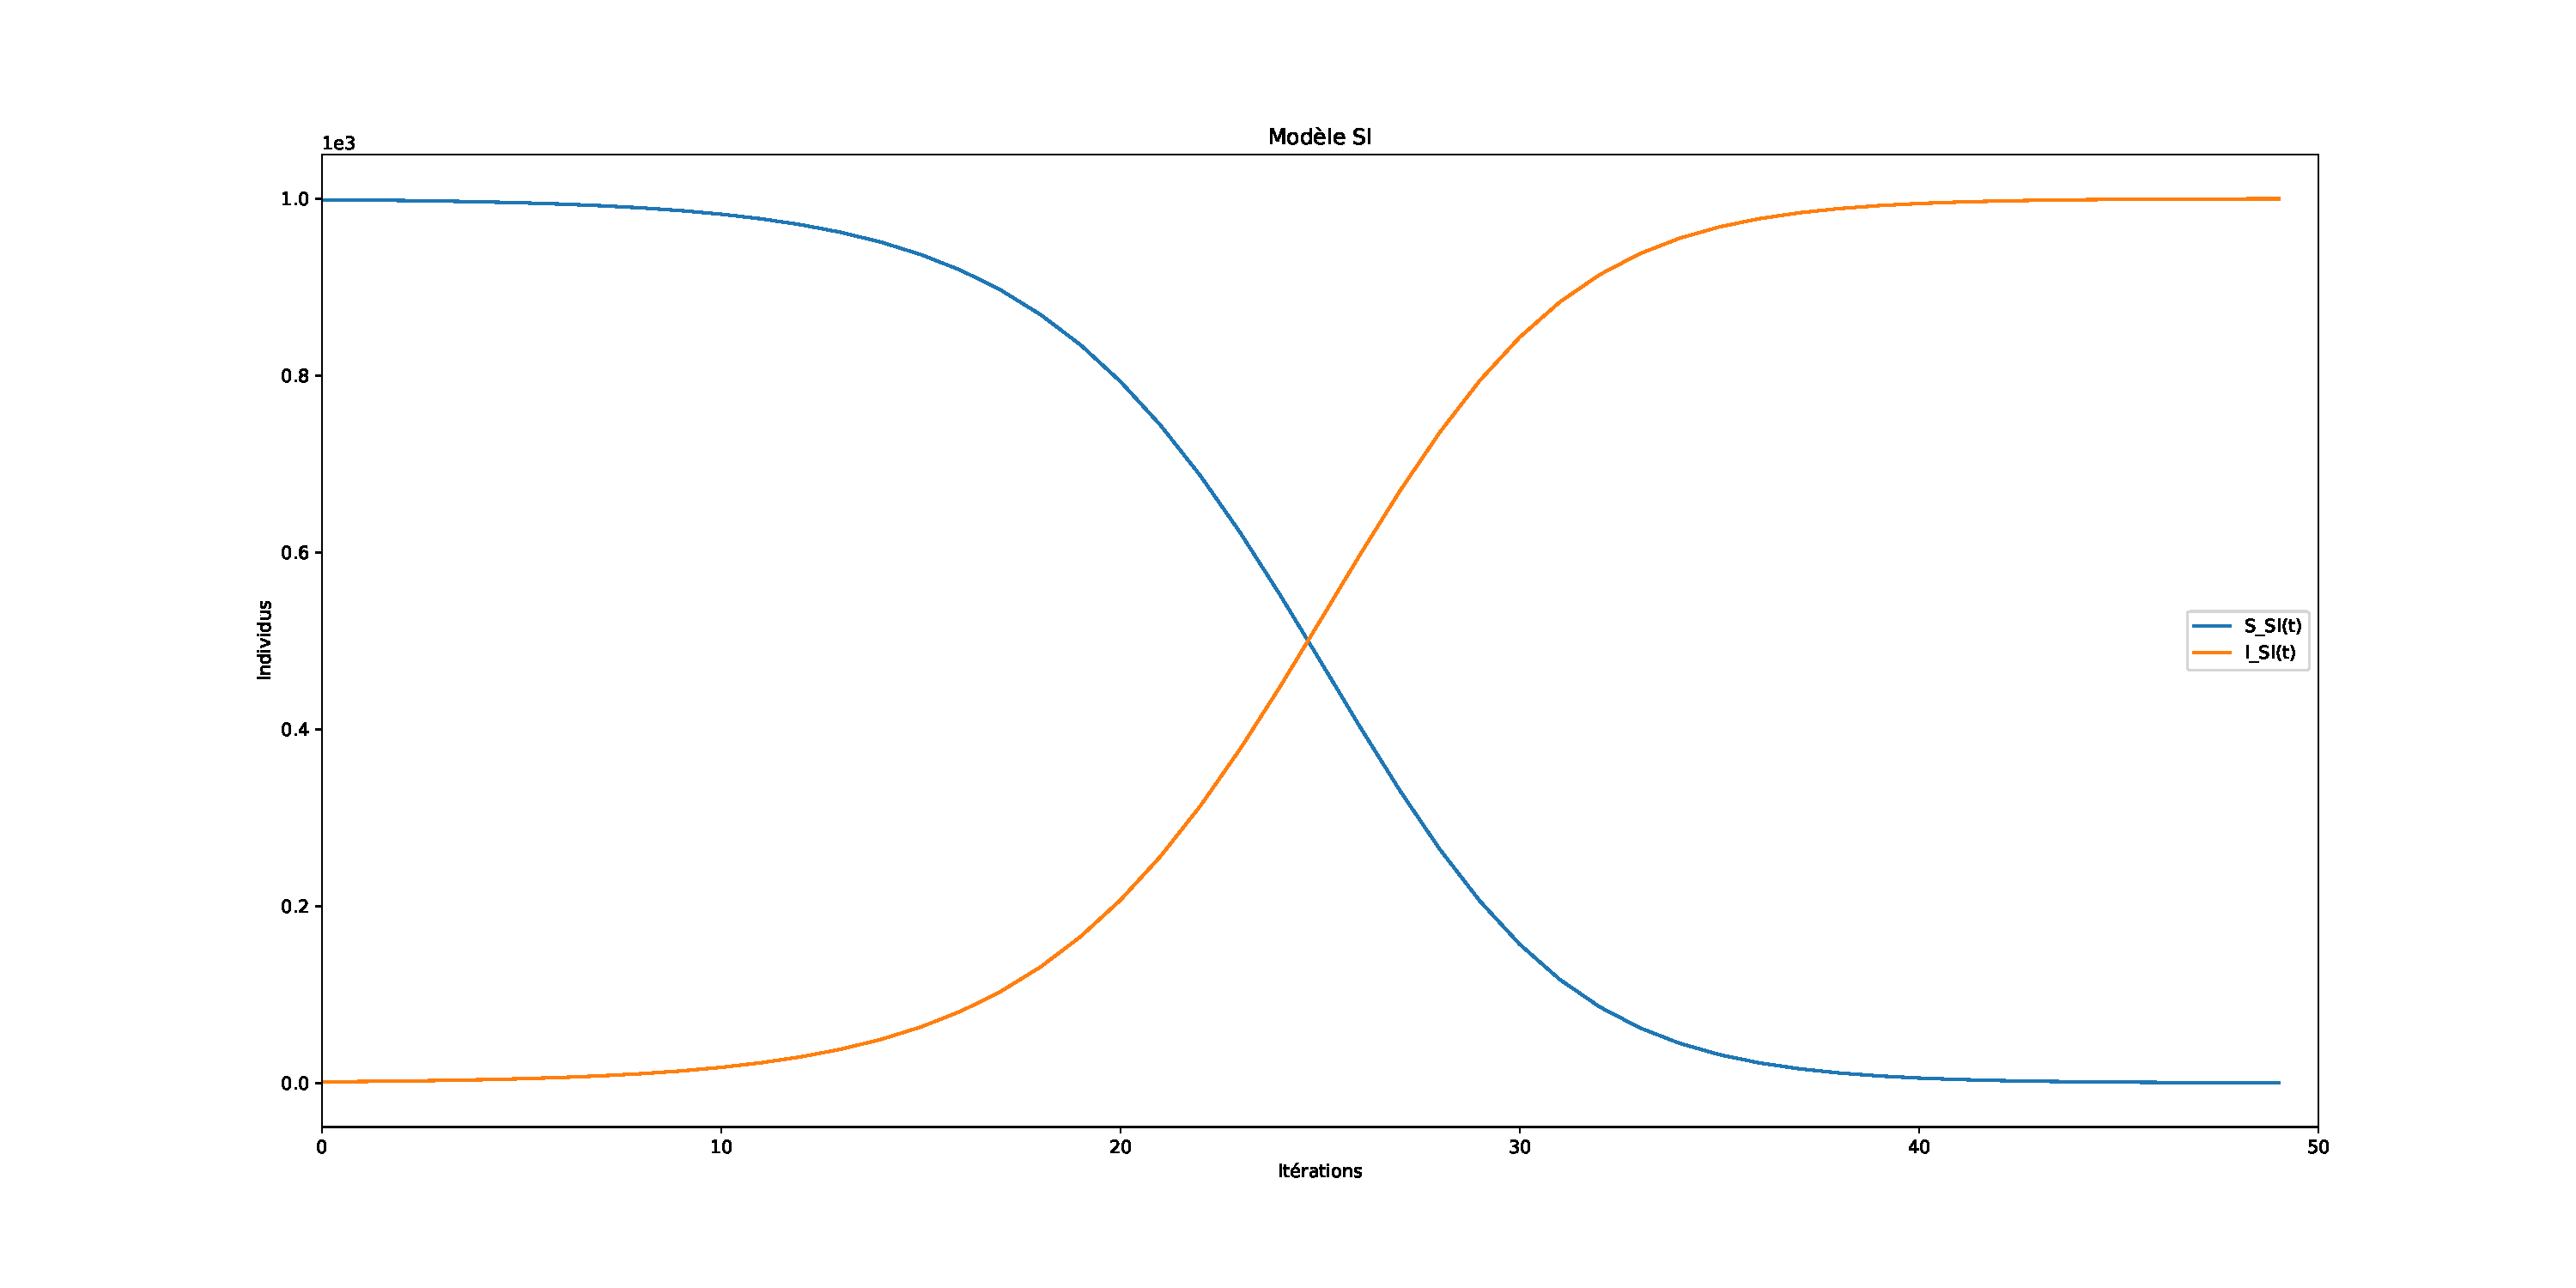
\includegraphics[width=1\textwidth]{Images/SI_exemple.pdf}
\caption[Modèle mathématique SI]{Modèle mathématique SI construit par les équations différentielles ordinaires. La courbe bleue représente le compartiment $S$ et la courbe orange le compartiment $I$}
\end{figure}

\section{Modèle SIR}

Les modèles compartimentaux SIR sont comparables aux modèles SI sauf qu'ils ont un compartiment supplémentaire $R$ incluant tous les individus guéris. Initialement les individus commencent dans le compartiment $S$ et passent dans le compartiment $I$ s'ils sont contaminés. Après une certaine période étant contaminés ils peuvent développer une immunité au pathogène et guérir. Tout individu développant une immunité à la maladie passe dans le dernier compartiment $R$ mais il est impossible de retourner dans le compartiment $S$. Ce modèle possède les mêmes paramètres que le modèle SI avec l'ajout d'une variable $\gamma$ positive définissant le taux de guérison.\\

Le modèle ayant trois compartiments, il est décrit par trois équations différentielles ordinaires.
\begin{align}
    \frac{dS}{dt} &= -\frac{\beta S I}{N}\\
    \frac{dI}{dt} &= \frac{\beta S I}{N} - \gamma I\\
    \frac{dR}{dt} &= \gamma I
\end{align}

Le modèle mathématique est très similaire au précédent. La différence vient du fait que certains individus du compartiment $I$ migrent vers $R$ à un certain rythme.\\

Comme pour le point précédent, python implémente les trois équations différentielles de la manière suivante :

\begin{minted}
[
frame=lines,
framesep=2mm,
baselinestretch=1.2,
bgcolor=LightGray,
fontsize=\footnotesize,
linenos
]
{Python}
S, I, R = S - beta * ((S * I) / N), I + beta * ((S * I) / N) - gamma * I, R + gamma * I 
\end{minted}

Les trois compartiments sont mis à jour à chaque pas de l'algorithme et ceci simultanément.\\

Une représentation graphique sur $100$ itérations avec les paramètres : $N = 1000, S = 999, I = 1, R = 0, \beta = 0.3, \gamma = 0.06$ :

\begin{figure}[h]
\centering
\captionsetup{justification=centering}
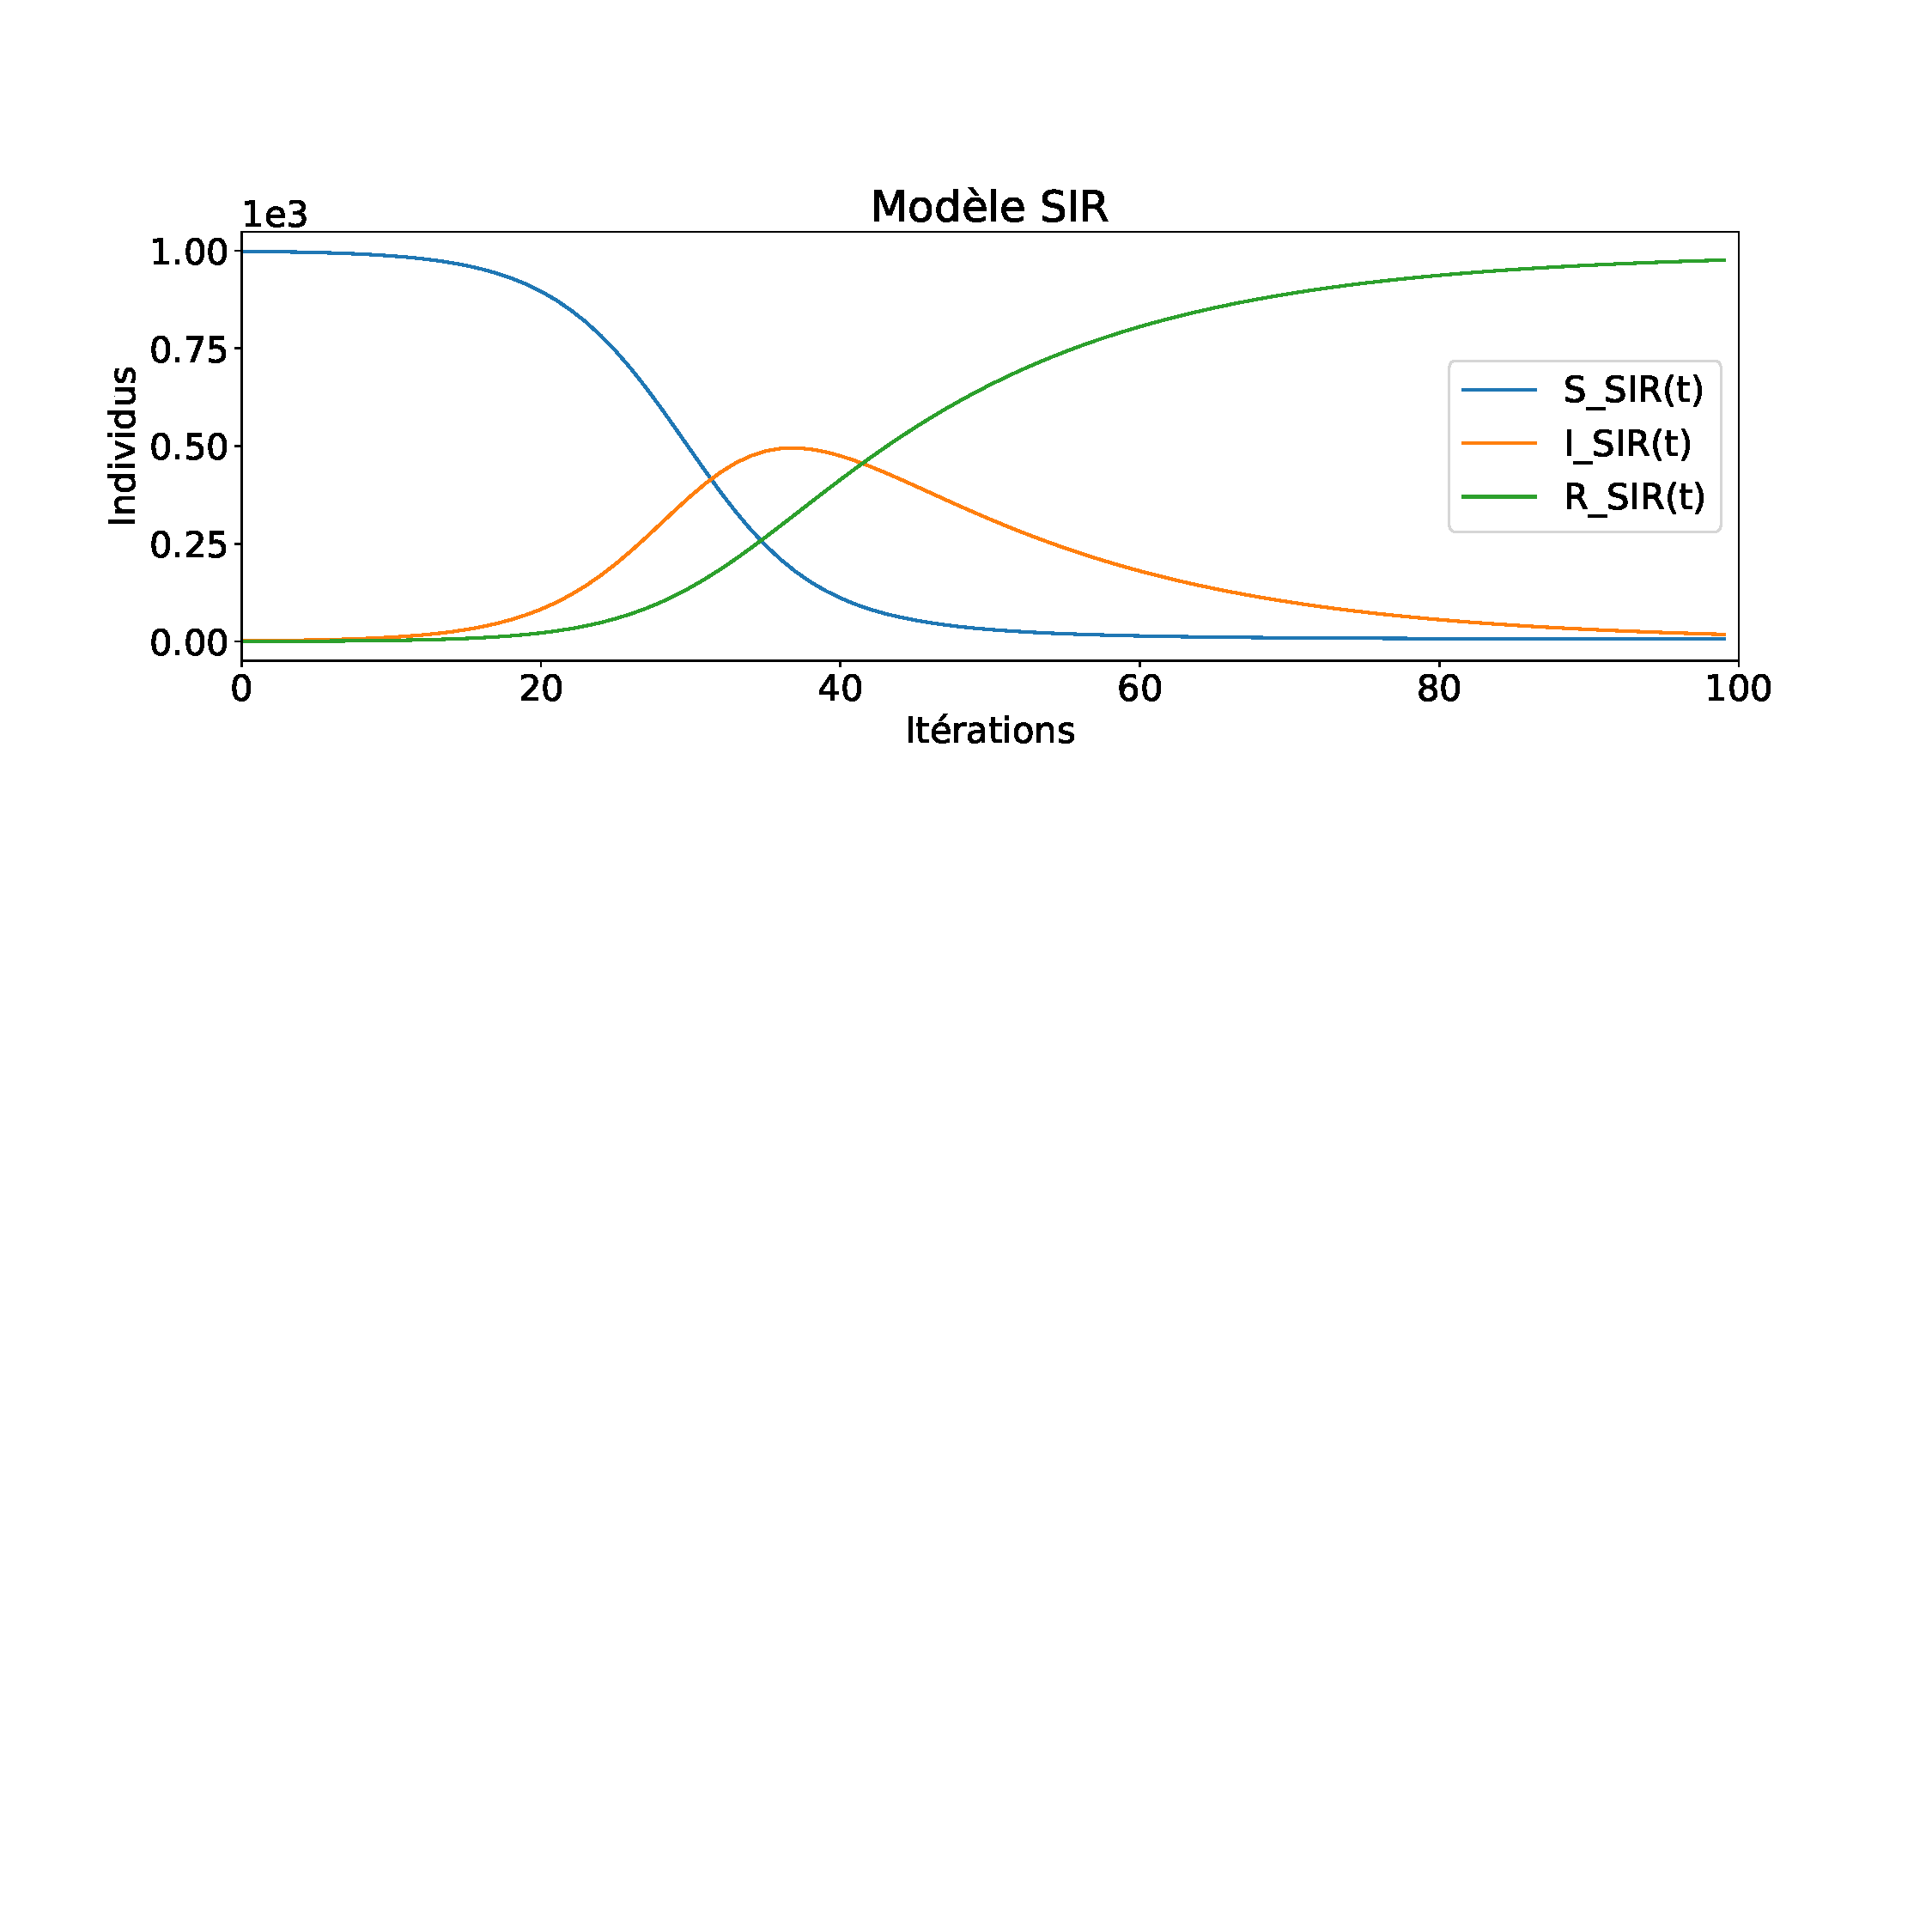
\includegraphics[width=1\textwidth]{Images/SIR_exemple.pdf}
\caption[Modèle mathématique SIR]{Modèle mathématique SIR construit par les équations différentielles ordinaires. La courbe bleue représente le compartiment $S$, la courbe orange le compartiement $I$ et finalement la courbe verte représente le compartiment $R$.}
\end{figure}

\section{Simulations de références}

Les modèles SI et SIR ont été prouvés par le passé et ont par conséquent une certaine validité. L'objectif ici est de valider notre modèle en le comparant aux résultats des modèles SI et SIR. Il s'agit donc de paramétrer notre modèle afin de le faire correspondre aux courbes des modèles valides déjà existant.\\

Notre modèle paramétré et validé par SI et SIR peut servir de référentiel pour des analyses. Ces simulations de base nous permettraient de quantifier les différences dans les résultats avec d'autres simulations paramétrées différemment. En effet une simulation crée son propre monde par conséquent un résultat seul ne révèle aucune information. Pour déduire des résultats de simulations il faut les comparer entre elles. C'est la raison pour laquelle nous établissons des simulations de références validée par SI et SIR.\\

Afin d'établir une référence nous paramétrons les variables des modèles SI et SIR ainsi que les paramètres de notre modèle. Une multitude de tailles de systèmes ainsi que de taille de population sont testées.\\

\subsection{Simulations de SI}

Dans ce chapitre nous essayons d'imiter des comportements décrits par le modèle SI. Notre modèle est paramétré en conséquence pour adopter les mêmes comportements que le modèle SI. L'objectif de cette section est de valider le modèle construit en montrant les similitudes dans les résultats avec le modèle SI déjà prouvé. \\

Les modèles compartimentaux n'ont pas de notion d'espace, c'est-à-dire que les individus du système n'ont pas de position géographique. Ces modèles considèrent tous les individus en contact les uns avec les autres et ceci modulé par le facteur $\beta$. Étant donné que notre modèle implémenté possède une notion d'espace, il a fallu l'adapter afin qu'il satisfasse les conditions des modèles compartimentaux. Deux solutions ont été trouvées pour palier à ce problème. La première est de désactiver la fonction de mouvement chez les individus et de la remplacer par une redistribution complète et aléatoire de toute la population. De ce fait nous redistribuons tous les individus et obtenons un mélange parfait à chaque itération. Cette méthode est appelée "perfect\_mix". La seconde méthode est de permettre aux individus du système de se déplacer davantage. Nous pouvons en effet simuler un mélange parfait en déplaçant un grand nombre de fois les individus à chaque itération. Initialement le modèle était conçu pour permettre à chaque itération à tous les individus de se déplacer d'une cellule. Mais un paramètre permet de déterminer le nombre de mouvements effectué par un individu par itération. Pour simuler le modèle SI le plus précisément possible il faut un grand nombre de déplacements. Ce nombre a été fixé à $1000$ ce qui signifie qu'un individu a le potentiel de se déplacer de $1000$ cellules en une seule itération.\\

Le modèle doit être paramétré spécifiquement pour adopter les mêmes comportements qu'un modèle SI. Un exemple de fichier de configuration est donné ci-dessous : 

\begin{minted}
[
frame=lines,
framesep=2mm,
baselinestretch=1.2,
bgcolor=LightGray,
fontsize=\footnotesize,
linenos
]
{C++}
TAILLE_SYSTEME = 200
NOMBRE_INDIVIDUS = 5000
ITERATIONS = 150
RERUN_LIMIT = 1000
FAIL_SEUIL = 10
GENOME_INIT_I = 0
GENOME_DIVERSITY_I = 0
GENOME_INIT_AP = 0
VITESSE_MUTATIONS_AP = 0
CHARGE_VIRALE = 1
PARAMETRE_FONCTION = 1
PARAMETRE_FONCTION_DOUBLE = 4
CELLULE_AP = 0
SURVIE_AP = 0
NOMBRE_MOUVEMENT = 1000
PERFECT_MIX = false
TEMPS_AVANT_IMMUNITE = 1
IMMUNITE_MECANISME = false
RESISTANCE_MECANISME = false
\end{minted}

Lorsqu'on veut simuler le modèle SI, il est nécessaire de désactiver la mécanique d'immunisation et de résistance naturelle.
\begin{minted}
[
frame=lines,
framesep=2mm,
baselinestretch=1.2,
bgcolor=LightGray,
fontsize=\footnotesize,
linenos
]
{C++}
IMMUNITE_MECANISME = false
RESISTANCE_MECANISME = false
\end{minted}

Il faut ensuite paramétrer le modèle en fonction de la simulation que nous cherchons à effectuer. Les paramètres principaux pour simuler le modèle SI sont donnés ci-dessous. Tous les autres paramètres du modèle ne sont pas révélateurs dans ces configurations.

\begin{minted}
[
frame=lines,
framesep=2mm,
baselinestretch=1.2,
bgcolor=LightGray,
fontsize=\footnotesize,
linenos
]
{C++}
TAILLE_SYSTEME = 200
NOMBRE_INDIVIDUS = 5000
ITERATIONS = 150
CHARGE_VIRALE = 1
CELLULE_AP = 0
NOMBRE_MOUVEMENT = 5000
PERFECT_MIX = false
IMMUNITE_MECANISME = false
RESISTANCE_MECANISME = false
\end{minted}

Pour toutes les mesures SI du document, les mécanismes de contaminations de cellules sont désactivés et le facteur de charge virale est par défaut à $1$.

\begin{minted}
[
frame=lines,
framesep=2mm,
baselinestretch=1.2,
bgcolor=LightGray,
fontsize=\footnotesize,
linenos
]
{C++}
CHARGE_VIRALE = 1
CELLULE_AP = 0
\end{minted}

Il reste ensuite à paramétrer la taille de la grille, le nombre d'individus, le nombre d'itérations et finalement le mode de déplacement. 


\subsection{Simulations de SIR}

Pour modéliser une situation reflétant un modèle SIR il faut un mécanisme d'immunités chez les individus. Notre modèle fournit un paramètre permettant d'activer ou de désactiver les processus d'immunités.

Un exemple de fichier de configuration pour simuler un modèle SIR est donné ci-dessous : 

\begin{minted}
[
frame=lines,
framesep=2mm,
baselinestretch=1.2,
bgcolor=LightGray,
fontsize=\footnotesize,
linenos
]
{C++}
TAILLE_SYSTEME = 200
NOMBRE_INDIVIDUS = 5000
ITERATIONS = 300
RERUN_LIMIT = 1000
FAIL_SEUIL = 10
GENOME_INIT_I = 65535
GENOME_DIVERSITY_I = 0
GENOME_INIT_AP = 0
VITESSE_MUTATIONS_AP = 0
CHARGE_VIRALE = 1
PARAMETRE_FONCTION = 4
PARAMETRE_FONCTION_DOUBLE = 4
CELLULE_AP = 0
SURVIE_AP = 0
NOMBRE_MOUVEMENT = 1000
PERFECT_MIX = false
TEMPS_AVANT_IMMUNITE = 1
IMMUNITE_MECANISME = true
RESISTANCE_MECANISME = false
\end{minted}

La différence entre la configuration d'un modèle SI et celle d'un modèle SIR est l'activation du mécanisme d'immunisation. Pour des questions de simplifications le paramètre de résistance naturelle est resté désactivé pour les simulations de SIR. D'autres paramètres comme les génomes ou le paramètre de fonction sont automatiquement activés par l'activation du paramètre d'immunisation :
\begin{minted}
[
frame=lines,
framesep=2mm,
baselinestretch=1.2,
bgcolor=LightGray,
fontsize=\footnotesize,
linenos
]
{C++}
IMMUNITE_MECANISME = true
\end{minted}

Pour simuler un modèle SIR classique il est aussi nécessaire de désactiver le mécanisme de mutation des agents pathogènes ainsi que le mécanisme de diversité chez les individus. Il reste ensuite à paramétrer les génomes initiaux, le paramètre de fonction ainsi que les autres paramètres du modèle.